
\documentclass[tikz,border=14pt]{standalone}
\usepackage{fontspec}
\usepackage{xeCJK}
\setmainfont{Liberation Serif}
\setsansfont{Liberation Sans}
\setmonofont{DejaVu Sans Mono}[Scale=0.82]
\setCJKmainfont{Noto Serif CJK SC}
\setCJKsansfont{Noto Serif CJK SC}
\setCJKmonofont{Noto Sans CJK SC}
\usepackage{amsmath,amssymb}
\usetikzlibrary{arrows.meta,calc}
\definecolor{ink}{HTML}{1E1E1E}
\definecolor{mid}{HTML}{5F5F5F}
\definecolor{hair}{HTML}{B0B0B0}
\definecolor{wash}{HTML}{F6F6F6}
\tikzset{
  line/.style={draw=ink,line width=0.55pt},
  softline/.style={draw=hair,line width=0.45pt},
  path/.style={draw=ink,line width=0.65pt,-{Latex[length=2.0mm,width=1.3mm]}},
  ctrl/.style={draw=mid,line width=0.55pt,dashed,-{Latex[length=1.75mm,width=1.2mm]}},
  smalltext/.style={font=\rmfamily\fontsize{8.7}{12.2}\selectfont,text=ink},
  dimtext/.style={font=\rmfamily\fontsize{8.15}{11.7}\selectfont,text=mid},
  code/.style={font=\ttfamily\fontsize{8.1}{11.6}\selectfont,text=ink},
  h/.style={font=\rmfamily\bfseries\fontsize{10.1}{14.0}\selectfont,text=ink},
  superh/.style={font=\rmfamily\bfseries\fontsize{14.4}{18.5}\selectfont,text=ink},
}

\begin{document}
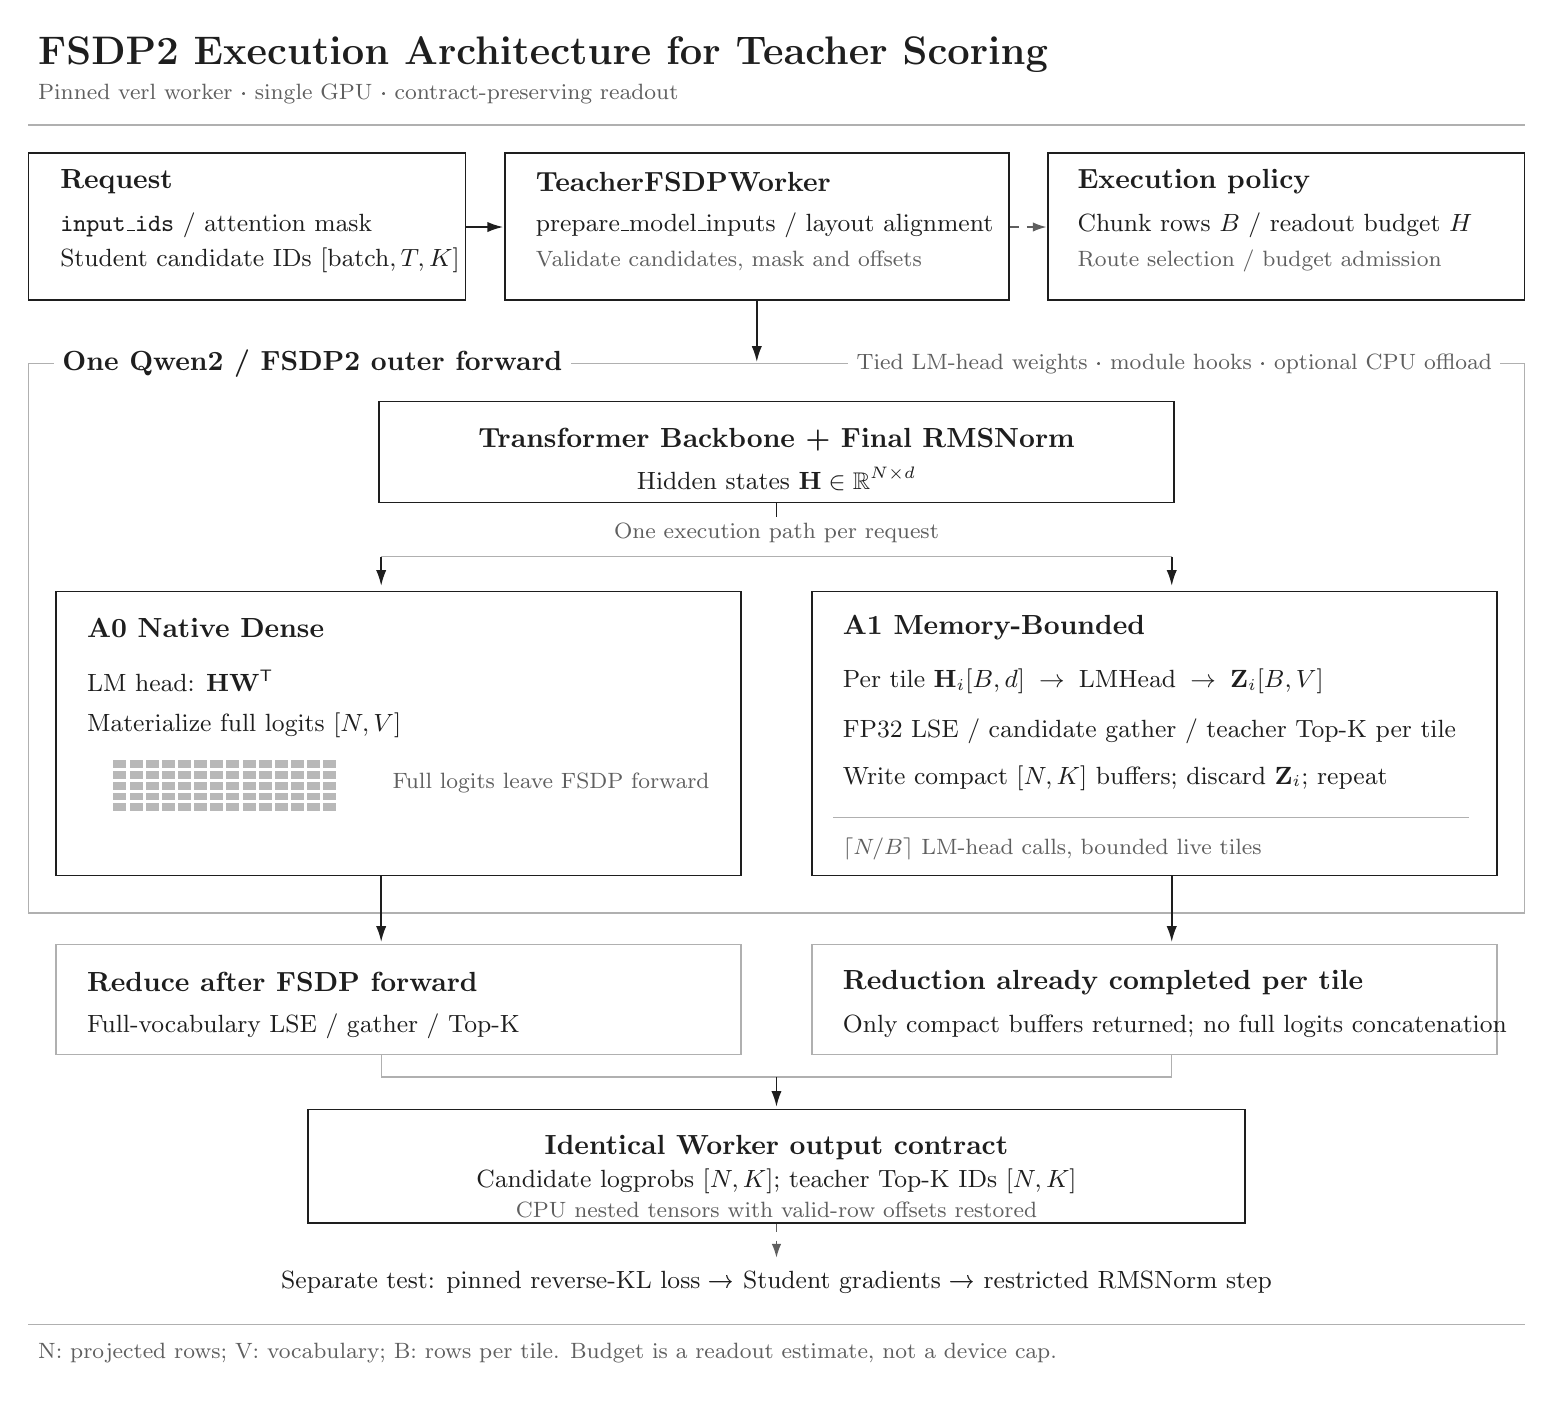
\begin{tikzpicture}[x=1cm,y=1.19cm]
  \node[superh,anchor=west] at (0,0) {FSDP2 Execution Architecture for Teacher Scoring};
  \node[dimtext,anchor=west] at (0,-0.42) {Pinned verl worker · single GPU · contract-preserving readout};
  \draw[softline] (0,-0.75) -- (19.0,-0.75);
  % Interface, adapter, planner are distinct: inputs flow, policy controls.
  \draw[line] (0,-1.05) rectangle (5.55,-2.62);
  \draw[line] (6.05,-1.05) rectangle (12.45,-2.62);
  \draw[line] (12.95,-1.05) rectangle (19,-2.62);
  \node[h,anchor=west] at (.28,-1.36) {Request};
  \node[smalltext,anchor=west] at (.28,-1.82) {\texttt{input\_ids} / attention mask};
  \node[smalltext,anchor=west] at (.28,-2.20) {Student candidate IDs $[\mathrm{batch},T,K]$};
  \node[h,anchor=west] at (6.32,-1.36) {TeacherFSDPWorker};
  \node[smalltext,anchor=west] at (6.32,-1.82) {prepare\_model\_inputs / layout alignment};
  \node[dimtext,anchor=west] at (6.32,-2.20) {Validate candidates, mask and offsets};
  \node[h,anchor=west] at (13.20,-1.36) {Execution policy};
  \node[smalltext,anchor=west] at (13.20,-1.82) {Chunk rows $B$ / readout budget $H$};
  \node[dimtext,anchor=west] at (13.20,-2.20) {Route selection / budget admission};
  \draw[path] (5.56,-1.84) -- (6.03,-1.84);
  \draw[ctrl] (12.47,-1.84) -- (12.93,-1.84);
  \draw[path] (9.25,-2.63) -- (9.25,-3.28);
  % FSDP boundary: the complete logits reduction in A0 is OUTSIDE this region.
  \draw[softline] (0,-3.30) rectangle (19,-9.16);
  \node[h,anchor=west,fill=white,inner sep=3pt] at (.32,-3.30) {One Qwen2 / FSDP2 outer forward};
  \node[dimtext,anchor=east,fill=white,inner sep=3pt] at (18.70,-3.30) {Tied LM-head weights · module hooks · optional CPU offload};
  \draw[line] (4.45,-3.70) rectangle (14.55,-4.78);
  \node[h] at (9.5,-4.11) {Transformer Backbone + Final RMSNorm};
  \node[smalltext] at (9.5,-4.53) {Hidden states $\mathbf H\in\mathbb R^{N\times d}$};
  \draw[path] (9.5,-4.78) -- (9.5,-5.17);
  \node[dimtext,fill=white,inner sep=2pt] at (9.5,-5.10) {One execution path per request};
  \draw[softline] (9.5,-5.36) -- (4.48,-5.36);
  \draw[softline] (9.5,-5.36) -- (14.52,-5.36);
  \draw[path] (4.48,-5.36) -- (4.48,-5.67);
  \draw[path] (14.52,-5.36) -- (14.52,-5.67);
  \draw[line] (.35,-5.73) rectangle (9.05,-8.76);
  \draw[line] (9.95,-5.73) rectangle (18.65,-8.76);
  \node[h,anchor=west] at (.62,-6.12) {A0  Native Dense};
  \node[smalltext,anchor=west] at (.62,-6.68) {LM head: $\mathbf H\mathbf W^\mathsf T$};
  \node[smalltext,anchor=west] at (.62,-7.16) {Materialize full logits $[N,V]$};
  % Technical matrix icon: purely schematic, one full N-by-V allocation.
  \foreach \i in {0,...,4}{\foreach \j in {0,...,13}{
    \fill[black!28] (1.08+\j*.205,-7.53-\i*.115) rectangle ++(.165,-.085);
  }}
  \node[dimtext,anchor=west] at (4.50,-7.77) {Full logits leave FSDP forward};
  \node[h,anchor=west] at (10.22,-6.12) {A1  Memory-Bounded};
  \node[smalltext,anchor=west] at (10.22,-6.69) {Per tile $\mathbf H_i[B,d]\;\to\;\mathrm{LMHead}\;\to\;\mathbf Z_i[B,V]$};
  \node[smalltext,anchor=west] at (10.22,-7.22) {FP32 LSE / candidate gather / teacher Top-K per tile};
  \node[smalltext,anchor=west] at (10.22,-7.72) {Write compact $[N,K]$ buffers; discard $\mathbf Z_i$; repeat};
  \draw[softline] (10.22,-8.14) -- (18.30,-8.14);
  \node[dimtext,anchor=west] at (10.22,-8.48) {$\lceil N/B\rceil$ LM-head calls, bounded live tiles};
  % Work moved across the FSDP boundary only in the Dense path.
  \draw[path] (4.48,-8.77) -- (4.48,-9.47);
  \draw[path] (14.52,-8.77) -- (14.52,-9.47);
  \draw[softline] (.35,-9.50) rectangle (9.05,-10.67);
  \draw[softline] (9.95,-9.50) rectangle (18.65,-10.67);
  \node[h,anchor=west] at (.62,-9.90) {Reduce after FSDP forward};
  \node[smalltext,anchor=west] at (.62,-10.37) {Full-vocabulary LSE / gather / Top-K};
  \node[h,anchor=west] at (10.22,-9.90) {Reduction already completed per tile};
  \node[smalltext,anchor=west] at (10.22,-10.37) {Only compact buffers returned; no full logits concatenation};
  \draw[softline] (4.48,-10.68) -- (4.48,-10.91) -- (9.50,-10.91);
  \draw[softline] (14.52,-10.68) -- (14.52,-10.91) -- (9.50,-10.91);
  \draw[path] (9.50,-10.91) -- (9.50,-11.23);
  \draw[line] (3.55,-11.26) rectangle (15.45,-12.47);
  \node[h] at (9.50,-11.66) {Identical Worker output contract};
  \node[smalltext] at (9.50,-12.02) {Candidate logprobs $[N,K]$; teacher Top-K IDs $[N,K]$};
  \node[dimtext] at (9.50,-12.33) {CPU nested tensors with valid-row offsets restored};
  \draw[ctrl] (9.50,-12.48) -- (9.50,-12.84);
  \node[smalltext] at (9.50,-13.10) {Separate test: pinned reverse-KL loss → Student gradients → restricted RMSNorm step};
  \draw[softline] (0,-13.55) -- (19,-13.55);
  \node[dimtext,anchor=west] at (0,-13.86) {N: projected rows; V: vocabulary; B: rows per tile. Budget is a readout estimate, not a device cap.};
\end{tikzpicture}
\end{document}
